% Provenance (never printed): see sources/outline_sources.md (Year 1: physical and chemical
% weathering; hydrolysis and its degrees; the ionic-potential diagram; clay minerals and
% climate; silicate weathering and carbon dioxide). Exercise and problem values in the Book 3
% scratch calculator calc/ch19.py; figure data from figdata/bachelor-1/ionic_potential.py and
% hydrolysis.py. Weathering is owned by Book 1 g5; chemical weathering, hydrolysis, clay mineral
% and laterite by Book 2 g10 (re-founded here). Silicate classes and the feldspars by ch. 7;
% Bowen's series by Book 2 g11; acid--base chemistry, solubility and oxidation by the chemistry
% books; soils and their horizons by the biology books. The silicate-weathering thermostat
% belongs to the Year 2 volume (told).
\chapter{风化与黏土}\label{ch:b1:weathering-clays}

老墓碑上的字迹逐渐褪去，字母锐利的棱角
被磨圆成浅浅的沟槽，大理石上的比板岩上的消失得更快。
一处坚硬得仿佛地球上无可比拟的花岗岩\omterm{def:b1:geological-maps:geological-map}{露头}，
其表面却会碎裂成粗砺的砂，从指缝间漏下，成为松散的颗粒：
玻璃质的石英、白垩状的\omterm{def:b1:rock-forming-minerals:groups}{长石}和片状\omterm{def:b1:rock-forming-minerals:groups}{云母}。在湿润的热带森林之下，
基岩可能埋藏很深，位于一层红色土壤之下，
这层土仍保留着岩石\omterm{def:b1:rock-forming-minerals:mineral}{矿物}的轮廓，却用铁锹就能挖开。
这三种现象都是地表水的作用。本章以化学的语言阐述这一作用：
哪些\omterm{def:b1:rock-forming-minerals:mineral}{矿物}最先被破坏，它们变成什么，为何有些元素随水流失而另一些
留下，气候如何决定结果，以及硅酸盐岩石的缓慢分解如何把
二氧化碳从
空气中夺走。

\begin{recall}
风化作用使岩石就地破碎（第~1~册，五年级）。\omterm{def:b1:weathering-clays:weathering}{化学
风化}改变\omterm{def:b1:rock-forming-minerals:mineral}{矿物}：\omterm{def:b1:rock-forming-minerals:groups}{长石}的\omterm{def:b1:weathering-clays:hydrolysis}{水解}生成一种\omterm{def:b1:weathering-clays:clay-mineral}{黏土
矿物}\omterm{def:b1:weathering-clays:clay-mineral}{高岭石}，并将钾和硅输入河流；\omterm{def:b1:weathering-clays:laterite}{红土}是
湿热气候下形成的红色、富铁富铝的产物（第~2~册，
十年级）。硅酸盐按 \ce{SiO4} 四面体如何共用顶角来分类，
\omterm{def:b1:rock-forming-minerals:silicate-classes}{层状硅酸盐}形成片层；\omterm{def:b1:rock-forming-minerals:groups}{长石}为含钠、钾、钙的\omterm{def:b1:rock-forming-minerals:silicate-classes}{架状硅酸盐}，
\omterm{def:b1:rock-forming-minerals:groups}{云母}为片状硅酸盐，片层之间夹有钾，
（见\cref{def:b1:rock-forming-minerals:silicate-classes}，
\cref{def:b1:rock-forming-minerals:groups}）。离子半径取决于
离子的电荷与配位数（见\cref{ch:b1:rock-forming-minerals}）。\omterm{def:b1:rock-forming-minerals:mineral}{矿物}
在冷却岩浆中按鲍文反应系列的顺序结晶，
\omterm{def:b1:rock-forming-minerals:groups}{橄榄石}最先、石英最后（第~2~册，十一年级）。酸释放氢
离子；溶于水的二氧化碳形成碳酸；氧化是
失去电子的过程；配平的方程式使每种元素和电荷都守恒
（化学各册）。土壤是按土层组织起来的生物层（
生物学各册）。
\end{recall}

\section{物理风化与化学风化}\label{sec:b1:weathering-clays:types}

在地下深处、高温高压且缺少游离水
与氧气的条件下形成的岩石，在地表处于非平衡状态。它以两种方式调整，
二者共同作用。

\begin{definition}[物理风化，化学风化]\label{def:b1:weathering-clays:weathering}
\emph{物理风化}\index{物理风化}是指岩石
原地破碎为较小碎块的过程，\omterm{def:b1:rock-forming-minerals:mineral}{矿物}成分不发生变化。
\emph{化学风化}\index{化学风化}是指岩石中的\omterm{def:b1:rock-forming-minerals:mineral}{矿物}在原地
与水及其携带的物质发生反应而实现的转变，
所携带的物质主要为氢离子、溶解的二氧化碳和氧气：有些\omterm{def:b1:rock-forming-minerals:mineral}{矿物}溶解，
另一些被地表稳定的新\omterm{def:b1:rock-forming-minerals:mineral}{矿物}所取代，
岩石的一部分则以溶液形式流失。
\end{definition}
% ledger: formoso:weathering

\emph{冰劈作用。}在 \qty{0}{\celsius} 时水的密度为
\qty{999.87}{kg.m^{-3}}，冰的密度为\qty{916.72}{kg.m^{-3}}：水冻结时体积膨胀
\qty{9.1}{\percent}。关于冰劈作用的旧观点是：
水在密闭裂隙中冻结并撑开裂隙，每次解冻和
冻结时都重复一次。花岗岩和大理石裂隙的一个模型，依据断裂力学
以及对冻结土的已有认识建立，则把重点放在别处：水
沿孔隙被吸引到裂隙中已有的冰体，正如它被吸向
冻结土壤中的冰透镜体一样，冰体不断长大并楔开裂隙，只要冻结持续，
这一过程便持续进行。持续冻结在约
\qty{-4}{\celsius}至\qty{-15}{\celsius}之间最为有效：温度更接近零度时，冰无法积累足够的压力，
而温度更低时，水已无法移动到冰体处。
% ledger: usgs:water-density, iapws:ice-density, wh85:frost

\emph{加热、卸荷与盐类。}反复的加热和冷却使
\omterm{def:b1:rock-forming-minerals:mineral}{矿物}膨胀量不同的岩石产生疲劳；被侵蚀带到地表的花岗岩
卸去上覆岩石的压力后膨胀，并沿平行地表的方向裂解成
薄板；蒸发的水中结晶出的盐类，
在沙漠和海岸地区撬开颗粒。

\omterm{def:b1:weathering-clays:weathering}{物理风化}的作用不止于破碎岩石：它还使岩石易受水的作用。

\begin{proposition}[破碎所打开的表面]\label{prop:b1:weathering-clays:surface}
边长为 $L$ 的立方体切成边长为 $L/n$ 的立方体后，
表面积变为原来的 $n$ 倍。一般地，质量为 $m$、密度为 $\rho$ 的颗粒，
边长都为 $d$，其表面积为 $S = 6m/(\rho d)$：比表面积 $S/m =
6/(\rho d)$ 与颗粒尺寸成反比。
\end{proposition}

\begin{proof}
边长为 $d$ 的立方体面积为 $6d^2$，质量为 $\rho d^3$，因此每个颗粒的
比表面积，以及任意多个颗粒的比表面积，都是 $6d^2/(\rho d^3)
= 6/(\rho d)$。将边长为 $L$ 的立方体切成 $n^3$ 个边长为 $L/n$ 的立方体，质量保持不变，
而 $d$ 除以 $n$，面积因此乘以 $n$。
\end{proof}

密度约为 \qty{2600}{kg.m^{-3}} 的一块\omterm{def:b1:rock-forming-minerals:groups}{长石}，其比表面积为
\qty{0.23}{m^2.kg^{-1}}（厘米级碎块）时，而
微米级颗粒为 \qty{2.3}{m^2.g^{-1}}，高出一万倍。化学
反应发生在表面，因此被冰劈碎裂或沿节理打开的岩石，
其\omterm{def:b1:weathering-clays:weathering}{化学风化}速度远快于完整的同种岩石。
% ledger: hom:albite, hom:orthoclase

\emph{化学反应。}方解石在含有二氧化碳的水中完全溶解，
这正是大理石墓碑失去字迹的原因
（第~2~册，十年级）。深色硅酸盐中的铁(II)被氧化为铁(III)，
生成的黄褐色和红色氧化物留存下来。其中最重要的无疑是\omterm{def:b1:weathering-clays:hydrolysis}{水解}，因为
硅酸盐构成了\omterm{def:b1:layered-earth:layers}{地壳}的大部分。氢离子来自
溶于水的二氧化碳——它从空气中溶入，又由根系和分解者
呼出进入土壤——以及腐烂植物的有机酸：
未受污染的地表水和土壤水的 pH 值介于 5.5 与 7 之间，
某些森林土壤有机层中的水可低至 3.5。水、温度、
表面积和酸度，因此是\omterm{def:b1:weathering-clays:weathering}{化学风化}的四个控制因素，
而温暖湿润的气候配以深厚的土壤，四者兼备。
% ledger: formoso:weathering

\section{硅酸盐的水解}\label{sec:b1:weathering-clays:hydrolysis}

\begin{definition}[硅酸盐的水解]\label{def:b1:weathering-clays:hydrolysis}
硅酸盐的\emph{水解}\index{水解（硅酸盐）}是指它与水和氢离子发生的
反应，其中氢离子取代金属阳离子，后者进入溶液；部分或全部硅
以溶解的硅酸 \ce{H4SiO4} 形式离开，\omterm{def:b1:rock-forming-minerals:mineral}{矿物}的其余部分重新构成
一种新的固体，即\omterm{def:b1:weathering-clays:clay-mineral}{黏土矿物}或氢氧化物。这种溶解是非一致的：
残留的固体，
其组成并不与被侵蚀的\omterm{def:b1:rock-forming-minerals:mineral}{矿物}相同。
\end{definition}
% ledger: formoso:weathering

铝是书写这一反应的关键：在土壤和河流的 pH 值下，
铝几乎不溶，固体产物将其全部保留，
其余一切均由此而定。

\begin{method}[配平水解反应]\label{met:b1:weathering-clays:balance}
已知被侵蚀的\omterm{def:b1:rock-forming-minerals:mineral}{矿物}与固体产物：
\begin{enumerate}
  \item 取产物的一个式单位，以及
        与之含有相同铝原子数的\omterm{def:b1:rock-forming-minerals:mineral}{矿物}量。
  \item \omterm{def:b1:rock-forming-minerals:mineral}{矿物}中未被产物利用的硅以 \ce{H4SiO4} 形式离开；
        未被产物利用的金属阳离子则以离子形式离开。
  \item 用左侧的氢离子平衡这些阳离子的电荷。
  \item 用左侧的水平衡氧。
  \item 检查氢：它必须自行平衡。若不平衡，则某个
        化学式有误。
  \item 若需要整数系数，则将各项同乘以适当的数。
\end{enumerate}
\end{method}

\begin{proposition}[长石的水解]\label{prop:b1:weathering-clays:feldspars}
以\omterm{def:b1:weathering-clays:clay-mineral}{蒙皂石}类\omterm{def:b1:rock-forming-minerals:mineral}{矿物}贝得石 \ce{Na_{0.5}Al2(Si_{3.5}Al_{0.5})O10(OH)2}
（略去层间水）、\omterm{def:b1:weathering-clays:clay-mineral}{高岭石} \ce{Al2Si2O5(OH)4} 与三水铝石
\ce{Al(OH)3} 为产物，
\begin{align*}
&\ce{5 NaAlSi3O8 + 4 H+ + 16 H2O -> 2 Na_{0.5}Al2(Si_{3.5}Al_{0.5})O10(OH)2 + 4 Na+ + 8 H4SiO4},\\ % ce-unbalanced-ok: decimal subscripts the checker cannot read; balance tested in tests/bachelor-1/test_weathering_clays.py
&\ce{2 NaAlSi3O8 + 2 H+ + 9 H2O -> Al2Si2O5(OH)4 + 2 Na+ + 4 H4SiO4},\\
&\ce{NaAlSi3O8 + H+ + 7 H2O -> Al(OH)3 + Na+ + 3 H4SiO4},\\
&\ce{CaAl2Si2O8 + 2 H+ + H2O -> Al2Si2O5(OH)4 + Ca^2+}.
\end{align*}
钠\omterm{def:b1:rock-forming-minerals:groups}{长石}在第一个反应中失去 \qty{80}{\percent} 的钠和 $8/15$ 的硅进入溶液，
在第二个反应中失去全部钠和 $2/3$ 的硅，
在第三个反应中两者全部失去。钙\omterm{def:b1:rock-forming-minerals:groups}{长石}失去全部钙，且
硅一点也不失去。
\end{proposition}
% ledger: webmineral:clays-b19, hom:albite, hom:anorthite

\begin{proof}
应用该方法。第一个反应：两个贝得石单位含有 $2\times2.5 = 5$
个铝，与 5 个钠\omterm{def:b1:rock-forming-minerals:groups}{长石}的铝相同；钠\omterm{def:b1:rock-forming-minerals:groups}{长石}的 15 个硅减去
$2\times3.5 = 7$ 个产物中的硅，余下 8 个 \ce{H4SiO4}；5 个钠减去 1 个，余下
4 个 \ce{Na+}，由 4 个 \ce{H+} 平衡；氧，左侧为 $40 + w$，右侧为 $24 + 32 =
56$，得 $w = 16$；氢，$4 + 32 = 36$ 与 $4 + 32 = 36$，校验无误。
第二个反应：2 个钠\omterm{def:b1:rock-forming-minerals:groups}{长石}提供\omterm{def:b1:weathering-clays:clay-mineral}{高岭石}的 2 个铝，余下 $6 - 2 = 4$
个 \ce{H4SiO4}、2 个 \ce{Na+} 与 2 个 \ce{H+}；氧 $16 + w = 9 + 16$，得 $w = 9$；
氢 $2 + 18 = 20 = 4 + 16$。第三个反应：1 个钠\omterm{def:b1:rock-forming-minerals:groups}{长石}、3 个硅酸、1 个
\ce{Na+} 与 1 个 \ce{H+}；氧 $8 + w = 3 + 12$，得 $w = 7$；氢
$1 + 14 = 15 = 3 + 12$。第四个反应：钙\omterm{def:b1:rock-forming-minerals:groups}{长石}的 2 个铝与 2 个硅恰为
\omterm{def:b1:weathering-clays:clay-mineral}{高岭石}所含，不产生硅酸，\ce{Ca^2+} 需 2 个 \ce{H+}；
氧 $8 + w = 9$，得 $w = 1$；氢 $2 + 2 = 4$。输出的比例即
溶液中的离子数与\omterm{def:b1:rock-forming-minerals:mineral}{矿物}中原子数之比：$4/5$ 与 $8/15$，然后
$2/2$ 与 $4/6$，再 $1/1$ 与 $3/3$。
\end{proof}

同一种钠\omterm{def:b1:rock-forming-minerals:groups}{长石}因而可以生成三种不同的固体，生成哪一种取决于
有多少水流经岩石并将产物带走：水少时，大部分硅和部分阳离子
留存下来，形成\omterm{def:b1:weathering-clays:clay-mineral}{蒙皂石}；水较多时，
只余下\omterm{def:b1:weathering-clays:clay-mineral}{高岭石}所需的硅；水极多时，
硅则全部离开。

\begin{definition}[双硅铝化、单硅铝化、铝铁化]\label{def:b1:weathering-clays:hydrolysis-degree}
硅酸盐\omterm{def:b1:weathering-clays:hydrolysis}{水解}的程度以其产物命名。
\emph{双硅铝化}\index{双硅铝化}形成 2:1 型\omterm{def:b1:weathering-clays:clay-mineral}{黏土矿物}，例如
\omterm{def:b1:weathering-clays:clay-mineral}{蒙皂石}，每个铝原子约含两个硅原子；部分阳离子留存其中。
\emph{单硅铝化}\index{单硅铝化}形成 1:1 型\omterm{def:b1:weathering-clays:clay-mineral}{黏土矿物}，即\omterm{def:b1:weathering-clays:clay-mineral}{高岭石}，每个铝原子
含一个硅原子；所有碱金属与碱土金属阳离子均被带走。
\emph{铝铁化}\index{铝铁化}则将硅全部除去，
留下氢氧化铝，即三水铝石。
\end{definition}
% ledger: pedron:stages, formoso:weathering

所达到的\omterm{def:b1:weathering-clays:hydrolysis}{水解}程度首先取决于气候，即降雨与温度，
其次取决于剖面的排水状况。在水更新缓慢之处，花岗岩
会失去大量的钠与钙，钾流失得较慢，
硅也只失去一部分：其\omterm{def:b1:rock-forming-minerals:groups}{长石}转化为 2:1 型黏土，并保留大量石英；
岩石崩解为石英、\omterm{def:b1:rock-forming-minerals:groups}{云母}及半风化\omterm{def:b1:rock-forming-minerals:groups}{长石}与黏土的混合砂。
在湿热热带的强降雨下，年降水量超过 \qty{2000}{mm}，
阳离子与硅被淋溶得多得多，
形成 Si/Al = 1 的\omterm{def:b1:weathering-clays:clay-mineral}{高岭石}。淋溶最强烈之处，
甚至\omterm{def:b1:weathering-clays:clay-mineral}{高岭石}中的硅也被带走，只剩下三水铝石。
% ledger: pedron:stages, goldich:1938, formoso:laterite

\begin{omfigure}
\begin{tikzpicture}[font=\small]
% fractions of albite's Na and Si exported by the three degrees (figdata/bachelor-1/hydrolysis.py)
\begin{axis}[width=10.5cm, height=6cm, ybar, bar width=0.5cm, ymin=0, ymax=112,
    xmin=0.45, xmax=3.55, xtick={1,2,3},
    xticklabels={{双硅铝化 \\ 至蒙皂石 \\ (Si/Al = 1.4)}, {单硅铝化 \\ 至高岭石 \\ (Si/Al = 1)}, {铝铁化 \\ 至三水铝石 \\ (Si/Al = 0)}},
    xticklabel style={align=center, font=\footnotesize},
    ylabel={溶液中输出量 (\si{\percent})}, ytick={0,20,...,100},
    legend style={at={(0.5,1.03)}, anchor=south, font=\footnotesize, legend columns=2, draw=none},
    nodes near coords={\pgfmathprintnumber[fixed,precision=0]{\pgfplotspointmeta}}, every node near coord/.append style={font=\scriptsize},
    enlarge x limits=false]
  \addplot[fill=omThm!60, draw=omThm!80!black] table[x=degree, y=Na] {figdata/out/bachelor-1-hydrolysis-degrees.dat};
  \addplot[fill=omDef!55, draw=omDef!80!black] table[x=degree, y=Si] {figdata/out/bachelor-1-hydrolysis-degrees.dat};
  \legend{钠, 硅}
\end{axis}
\end{tikzpicture}

{\small 钠\omterm{def:b1:rock-forming-minerals:groups}{长石}\omterm{def:b1:weathering-clays:hydrolysis}{水解}的三个程度：溶液中被带走的钠的百分比，
以及被带走的硅的百分比，二者均由配平的
反应式算得，以及残留固体中硅与铝之比。铝
在三种情形下都完全留在固体中。}
\label{fig:b1:weathering-clays:degrees}
\end{omfigure}


\begin{omfigure}
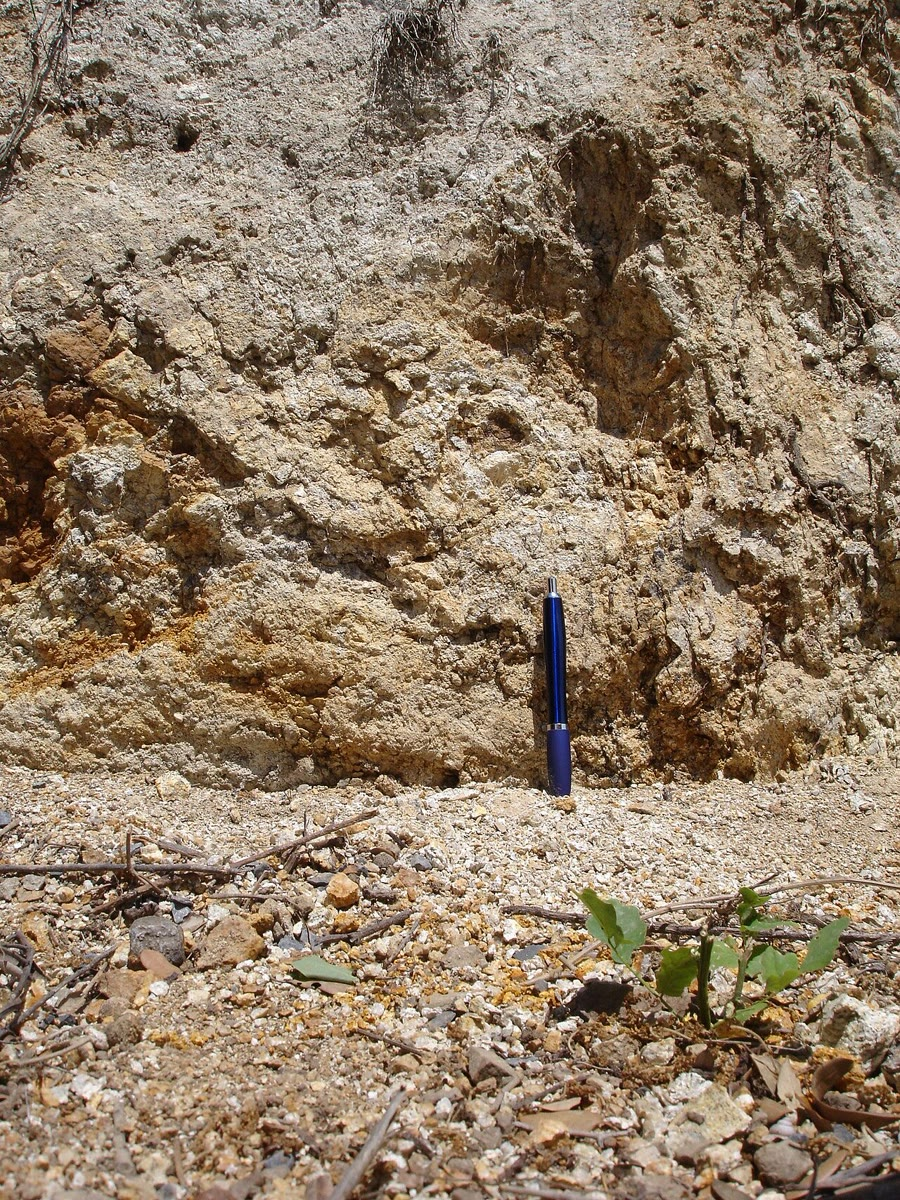
\includegraphics[height=6.3cm]{images/book3/b1-granite-grus.jpg}\hfill
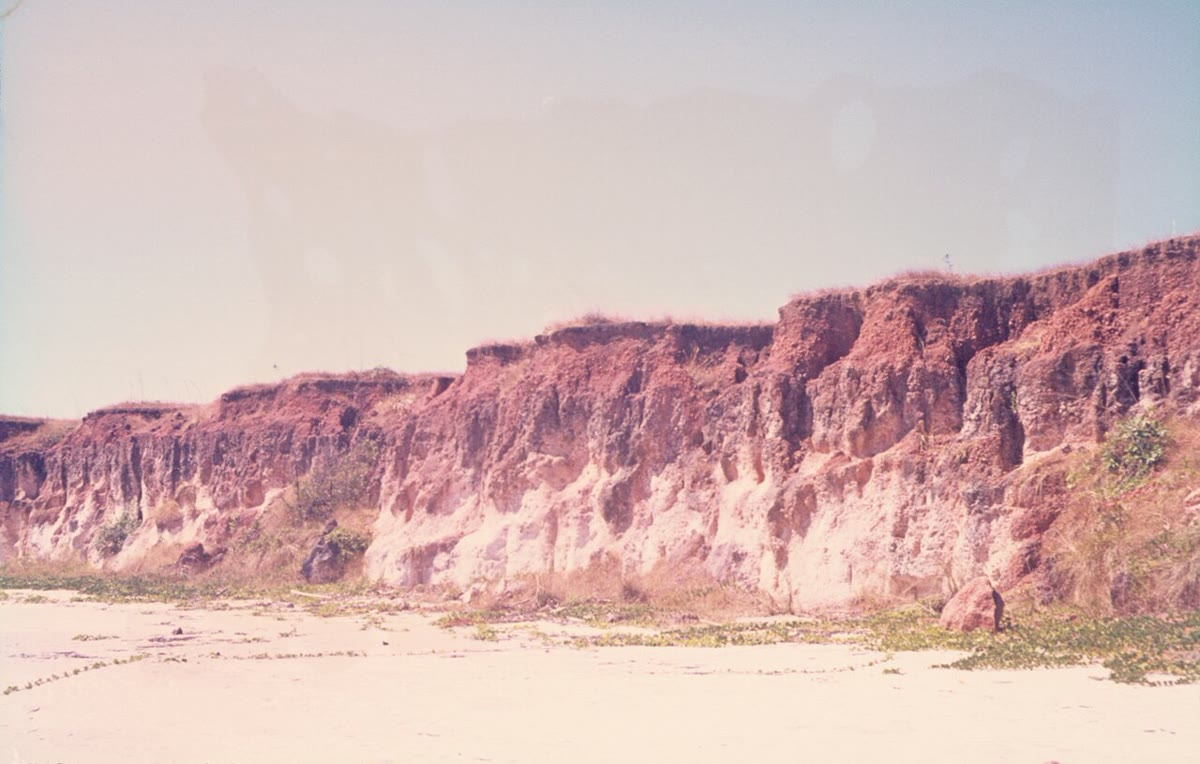
\includegraphics[height=6.3cm]{images/book3/b1-bauxite-weipa.jpg}
\par\smallskip{\small 左：比利牛斯山的风化花岗岩，仍在原地，但
正碎裂为石英、\omterm{def:b1:rock-forming-minerals:groups}{长石}和\omterm{def:b1:rock-forming-minerals:groups}{云母}构成的沙，松散的沙堆位于其
脚下；笔给出了比例尺。照片：Pinpin，CC~BY~2.5。右：
澳大利亚北部韦帕海岸上的风化剖面：红色铝土矿，
即\omterm{def:b1:weathering-clays:hydrolysis-degree}{铝铁化}的产物，覆于富含\omterm{def:b1:weathering-clays:clay-mineral}{高岭石}的白色砂岩之上。照片：
Werner Schellmann，1969，CC~BY-SA~2.5。均来自维基共享资源。}
\label{fig:b1:weathering-clays:photos}
\end{omfigure}
% ledger: commons:grus, commons:weipa

\emph{哪种\omterm{def:b1:rock-forming-minerals:mineral}{矿物}先被风化。}1938 年，塞缪尔·戈尔迪奇比较风化剖面与其母岩，
提出了一个\omterm{def:b1:rock-forming-minerals:mineral}{矿物}序列，按其在风化中由最不稳定至最稳定排列，
并发现该序列遵循\omterm{def:b1:rock-forming-minerals:mineral}{矿物}自岩浆中结晶的顺序：
即\omterm{def:b1:rock-forming-minerals:groups}{橄榄石}与富钙\omterm{def:b1:rock-forming-minerals:groups}{斜长石}最先，
石英最后。在最高温度下形成的\omterm{def:b1:rock-forming-minerals:mineral}{矿物}，
在地表最远离平衡。现代排序自最不耐风化至
最耐风化，其列为：黄铁矿、方解石、白云石、\omterm{def:b1:rock-forming-minerals:groups}{橄榄石}、钙质
\omterm{def:b1:rock-forming-minerals:groups}{斜长石}、\omterm{def:b1:rock-forming-minerals:groups}{辉石}、中等\omterm{def:b1:rock-forming-minerals:groups}{斜长石}、\omterm{def:b1:rock-forming-minerals:groups}{角闪石}、黑\omterm{def:b1:rock-forming-minerals:groups}{云母}、
钾\omterm{def:b1:rock-forming-minerals:groups}{长石}、白\omterm{def:b1:rock-forming-minerals:groups}{云母}、\omterm{def:b1:weathering-clays:clay-mineral}{蒙皂石}、石英、\omterm{def:b1:weathering-clays:clay-mineral}{高岭石}，以及氧化物
三水铝石和赤铁矿。溶解速率的实验测量证实了该排序；
但它仍只是一种排序，而非定律，因为每种\omterm{def:b1:rock-forming-minerals:mineral}{矿物}的速率
还取决于其周围的水。风化的最终产物，
\omterm{def:b1:weathering-clays:clay-mineral}{高岭石}、三水铝石和赤铁矿，是其中最耐风化的：它们
在地表本已稳定。
% ledger: goldich:1938, formoso:weatherability, lasaga:1984

\emph{风化剖面的质量平衡。}风化会带走物质，因此在风化岩石中测得的
浓度并不能说明损失了多少：
其他元素的流失使留下的元素浓缩。一种不移动的
元素可作为参照。

\begin{proposition}[不移动元素的质量平衡]\label{prop:b1:weathering-clays:immobile}
设 $i$ 为风化不会迁移的元素，其在母岩与风化岩石中的质量分数
分别为 $C_{i,p}$ 与 $C_{i,w}$。则一定质量
$m_p$ 的母岩变为质量 $m_w = m_p C_{i,p}/C_{i,w}$ 的风化岩石，
而任一其他元素 $j$ 的损失比例为
\[
  f_j = 1 - \frac{C_{j,w}}{C_{j,p}}\,\frac{C_{i,p}}{C_{i,w}} .
\]
\end{proposition}

\begin{proof}
元素 $i$ 的质量守恒：$m_p C_{i,p} = m_w C_{i,w}$，由此得 $m_w$。
元素 $j$ 的质量由 $m_p C_{j,p}$ 变为 $m_w C_{j,w}$，
其残留比例为 $m_w C_{j,w}/(m_p C_{j,p}) = (C_{j,w}/C_{j,p})(C_{i,p}/C_{i,w})$，
$f_j$ 即为一减去该残留比例。
\end{proof}

通常选用钛和锆，其理由
由下一节给出。

\section{哪些元素流失：离子势}\label{sec:b1:weathering-clays:ionic}

钠、钾和钙随水流失；铝、铁（III）和
钛留下；硅介于两者之间。区别在于每种离子
在水中的行为不同。

\begin{definition}[离子势]\label{def:b1:weathering-clays:ionic-potential}
一个离子的\emph{离子势}\index{离子势}为 $z/r$，
即其电荷数 $z$ 与离子半径 $r$ 之比，这里以埃为单位（所有离子取相同配位数，
下文均取六配位）。
\end{definition}
% ledger: nomad:goldschmidt, dangic:goldschmidt, shannon:radii-b19

\begin{proposition}[离子势的三个区间]\label{prop:b1:weathering-clays:fields}
在风化水中，$z/r < 3$ 的离子以水合阳离子形式
留在溶液中并被带走（可溶阳离子）；$3 < z/r < 10$ 的离子
与水中的氢氧根离子结合，在释放处以氢氧化物或氧化物
沉淀（\omterm{def:b1:weathering-clays:hydrolysis}{水解}产物）；$z/r > 10$ 的离子与氧结合得如此紧密，
以至于排斥氢离子，并以可溶的含氧酸根形式迁移，例如
碳酸根、硫酸根、磷酸根和硝酸根。硅在 $z/r = 10$ 处，位于
边界上，其部分被淋滤，风化越强，淋滤越多。
\end{proposition}
\admitted
% ledger: nomad:goldschmidt, dangic:goldschmidt

该规律是经验性的，由维克托·莫里茨·戈尔德施密特于 20 世纪 30 年代提出，
其边界只是近似的；其背后的化学原理，即阳离子与其周围水分子中氧之间的吸引，
属于化学教材的内容。一个小而高电荷的阳离子会强烈拉扯
其水分子中的电子，以至于水分子失去一个氢离子而变为氢氧根：
程度适中时，氢氧根沉淀；程度极强时，
连氢氧根也失去其中的氢，
留下含氧酸根。

下图一目了然地展示了岩石的风化。钠（$z/r = 0.98$）、
钾（0.72）、钙（2.0）和镁（2.8）流失：它们是
河水和海水中的阳离子。铝（5.6）、铁（III）（4.7）、钛
（6.6）和锆（5.6）留下，并在风化最强的剖面中富集；
钛和锆此外还赋存于几乎不风化的\omterm{def:b1:rock-forming-minerals:mineral}{矿物}中，
是\cref{prop:b1:weathering-clays:immobile}中的不移动参照元素。硅
（10.0）是其部分流失定义\omterm{def:b1:weathering-clays:hydrolysis}{水解}程度的元素。
% ledger: shannon:radii-b19

氧化会使离子越过边界。铁（II）的 $z/r = 2.6$，是
可溶阳离子；铁（III）为 4.7，属于\omterm{def:b1:weathering-clays:hydrolysis}{水解}产物。在无氧的渍水土壤中，
铁以 \ce{Fe^2+} 的形式溶解并被带走，留下灰色
土壤；而水与空气相遇处，如泉眼或排水良好的土壤中，
铁被氧化，并立即以红色和褐色氧化物的形式沉淀。锰
的行为相同：\ce{Mn^2+}（2.4）对 \ce{Mn^4+}（7.5）。
% ledger: nomad:goldschmidt, shannon:radii-b19

\begin{omfigure}
\begin{tikzpicture}[font=\small]
% ionic-potential diagram (figdata/bachelor-1/ionic_potential.py): charge against Shannon radius
\begin{axis}[width=12.5cm, height=8.4cm, xmin=0, xmax=1.8, ymin=0, ymax=7,
    xlabel={离子半径 $r$（\si{\angstrom}，六配位）}, ylabel={电荷 $z$},
    ytick={1,...,6}, xtick={0,0.2,...,1.8}, xticklabel style={/pgf/number format/fixed},
    axis on top, clip=true]
  \fill[omThm!14] (axis cs:0,0) -- (axis cs:1.8,0) -- (axis cs:1.8,5.4) -- cycle;
  \fill[omDef!16] (axis cs:0,0) -- (axis cs:1.8,5.4) -- (axis cs:1.8,7) -- (axis cs:0.7,7) -- cycle;
  \fill[omExo!18] (axis cs:0,0) -- (axis cs:0.7,7) -- (axis cs:0,7) -- cycle;
  \addplot[black, thick] table[x=r, y=z3] {figdata/out/bachelor-1-ionic_potential-lines.dat};
  \addplot[black, thick] table[x=r, y=z10] {figdata/out/bachelor-1-ionic_potential-lines.dat};
  \addplot[only marks, mark=*, mark size=1.6pt, black,
      point meta=explicit symbolic, nodes near coords,
      visualization depends on={value \thisrow{anc} \as \anc},
      every node near coord/.append style={font=\scriptsize, inner sep=2.6pt, anchor=\anc}]
    table[x=r, y=z, meta=tex] {figdata/out/bachelor-1-ionic_potential-ions.dat};
  \node[font=\footnotesize, align=center, fill=white, fill opacity=0.8, text opacity=1, rounded corners=1pt] at (axis cs:1.45,2.75) {可溶阳离子 \\ $z/r < 3$};
  \node[font=\footnotesize, align=center, fill=white, fill opacity=0.8, text opacity=1, rounded corners=1pt] at (axis cs:1.15,6.3) {水解产物 \\ $3 < z/r < 10$};
  \node[font=\footnotesize, align=left, fill=white, fill opacity=0.8, text opacity=1, rounded corners=1pt, anchor=north west] at (axis cs:0.015,6.95) {可溶含氧阴离子，$z/r > 10$};
  \node[font=\scriptsize, rotate=28, anchor=south] at (axis cs:1.62,4.86) {$z/r = 3$};
  \node[font=\scriptsize, rotate=61, anchor=south] at (axis cs:0.2,2.0) {$z/r = 10$};
\end{axis}
\end{tikzpicture}

{\small \omterm{def:b1:weathering-clays:ionic-potential}{离子势}图：每种离子按其六配位下的有效离子
半径（Shannon，1976）与电荷定位。直线
$z/r = 3$ 和 $z/r = 10$ 将以阳离子形式进入溶液的离子、
留在氢氧化物或氧化物中的离子，以及以含氧阴离子形式迁移的离子分开。
硅位于上边界上。}
\label{fig:b1:weathering-clays:ionic-potential}
\end{omfigure}
% ledger: shannon:radii-b19, nomad:goldschmidt

\section{黏土矿物}\label{sec:b1:weathering-clays:clays}

\begin{definition}[黏土矿物、高岭石、伊利石、蒙皂石、绿泥石]\label{def:b1:weathering-clays:clay-mineral}
称\emph{黏土矿物}\index{黏土矿物}为含水铝
\omterm{def:b1:rock-forming-minerals:silicate-classes}{层状硅酸盐}，通常为直径几微米或更小的颗粒，其结构由
四面体层（T）与八面体层（O）组合构成的层。四面体层由共用三个角的 \ce{SiO4} 四面体组成，
八面体层由铝或镁构成，并被氧和羟基包围。
在\emph{高岭石}\index{高岭石}，
\ce{Al2Si2O5(OH)4}，每层由一个 T 层和一个 O 层构成（1:1 型，即 T--O 层），
不带电，层间靠氢键结合。2:1 型（T--O--T）
黏土\omterm{def:b1:rock-forming-minerals:mineral}{矿物}中，O 层夹在两层 T 层之间，两层 T 层均朝向它：
\emph{伊利石}\index{伊利石}为不膨胀的 2:1 型黏土\omterm{def:b1:rock-forming-minerals:mineral}{矿物}，层间有钾
离子，类似于含钾较少的\omterm{def:b1:rock-forming-minerals:groups}{云母}；
\emph{蒙皂石}\index{蒙皂石}为 2:1 型黏土\omterm{def:b1:rock-forming-minerals:mineral}{矿物}，层间具水合的
可交换阳离子与水，层间能吸收更多的水
而膨胀；\emph{绿泥石}\index{绿泥石}为 2:1 型\omterm{def:b1:rock-forming-minerals:mineral}{矿物}，其
带负电的层与带正电的八面体层交替排列，
八面体层为水镁石型 \ce{(Mg,Fe)(OH)2}，并含少量铝。
\end{definition}
% ledger: usgs:clay-groups, usgs:clay-settings, webmineral:clays-b19, biscaye:1965

层的电荷决定各层如何堆叠，电荷来自
片层中的取代（见\cref{def:b1:rock-forming-minerals:substitution}）。

\begin{proposition}[2:1 型层的电荷]\label{prop:b1:weathering-clays:layer-charge}
化学式为 $\mathrm{(Si_{4-x}Al_x)(Al_{2-y}Mg_y)O_{10}(OH)_2}$ 的 2:1 型层，其中
四面体层中有 $x$ 个铝取代硅，八面体层中有 $y$ 个镁
取代八面体层中的铝，每化学式单位
带电荷 $-(x + y)$。
\end{proposition}

\begin{proof}
将电荷相加：四面体阳离子的贡献为 $4(4 - x) + 3x$，
八面体阳离子贡献 $3(2 - y) + 2y$，氧贡献 $-2\times10$，羟基贡献 $-1\times2$，
合计：$16 - x + 6 - y - 20 - 2 = -(x + y)$。
\end{proof}

无取代（$x = y = 0$）时该层呈电中性，如
\ce{Al2Si4O10(OH)2}，即叶蜡石，层间仅靠
较弱的作用力结合。
在白\omterm{def:b1:rock-forming-minerals:groups}{云母}中，$x = 1$，电荷 $-1$ 由一个钾离子平衡，该钾离子
将各层锁合在一起；\omterm{def:b1:weathering-clays:clay-mineral}{伊利石}与之接近，钾含量略少。
在\cref{prop:b1:weathering-clays:feldspars}所述的贝得石中，$x = 0.5$：电荷
$-0.5$ 由 $0.5$ 个钠离子平衡。电荷越小，层间结合
越松，层间可进入水和水合阳离子，这就是为什么
\omterm{def:b1:weathering-clays:clay-mineral}{蒙皂石}的电荷约为每化学式单位 0.3 至 0.5，
如蒙脱石和贝得石的化学式所示，它会膨胀，而\omterm{def:b1:weathering-clays:clay-mineral}{伊利石}不会。
\omterm{def:b1:weathering-clays:clay-mineral}{蒙皂石}的层间阳离子可交换，各常见\omterm{def:b1:weathering-clays:clay-mineral}{黏土矿物}的交换容量
取决于其结构：\omterm{def:b1:weathering-clays:clay-mineral}{高岭石}（层不带电）的交换容量为 3 至 15 毫当量每
\qty{100}{g}，\omterm{def:b1:weathering-clays:clay-mineral}{伊利石}为 10 至 40，
蒙脱石（一种\omterm{def:b1:weathering-clays:clay-mineral}{蒙皂石}）为 70 至 100。钾能锁定\omterm{def:b1:rock-forming-minerals:groups}{云母}的层，有利于
形成\omterm{def:b1:weathering-clays:clay-mineral}{伊利石}；\omterm{def:b1:weathering-clays:clay-mineral}{蒙皂石}形成于钾缺乏而
钙、镁充足的环境。
% ledger: webmineral:clays-b19, carroll:cec, usgs:clay-settings

\begin{omfigure}
\begin{tikzpicture}[font=\footnotesize, >={Stealth[length=4pt]}, y=0.2cm, x=1cm]
% schematic clay-mineral structures, vertical scale proportional to the basal spacings
% (USGS OFR 01-041, ledger usgs:clay-xrd): kaolinite 7, illite 10, smectite 14 (air-dried), chlorite 14 angstrom.
% T sheet 2 A thick, O sheet 2.4 A thick (schematic); the column width is 2.2 cm.
\def\W{2.2}
\newcommand{\Tsheet}[1]{% tetrahedral sheet whose base is at y=#1
  \fill[omDef!35] (0,#1) rectangle (\W,#1+2);
  \foreach \i in {0,...,6} {\draw[omDef!80!black, line width=0.4pt] (0.04+\i*0.31,#1) -- (0.195+\i*0.31,#1+2) -- (0.35+\i*0.31,#1) -- cycle;}
}
\newcommand{\TsheetDown}[1]{% inverted tetrahedral sheet, base at the top (y=#1+2)
  \fill[omDef!35] (0,#1) rectangle (\W,#1+2);
  \foreach \i in {0,...,6} {\draw[omDef!80!black, line width=0.4pt] (0.04+\i*0.31,#1+2) -- (0.195+\i*0.31,#1) -- (0.35+\i*0.31,#1+2) -- cycle;}
}
\newcommand{\Osheet}[2]{% octahedral sheet, base at y=#1, fill colour #2
  \fill[#2] (0,#1) rectangle (\W,#1+2.4);
  \foreach \i in {0,...,4} {\draw[black!55, line width=0.4pt] (0.17+\i*0.42,#1+1.2) -- ++(0.17,1.0) -- ++(0.17,-1.0) -- ++(-0.17,-1.0) -- cycle;}
}
\newcommand{\spacing}[3]{% arrow for d001 from y=#1 to y=#2 with label #3
  \draw[<->, line width=0.5pt] (\W+0.18,#1) -- (\W+0.18,#2) node[midway, right, inner sep=2pt] {#3};
  \draw[black!40, densely dotted] (\W,#1) -- (\W+0.28,#1); \draw[black!40, densely dotted] (\W,#2) -- (\W+0.28,#2);
}
% ---------- kaolinite: T-O, d = 7.2
\begin{scope}[xshift=0cm]
  \foreach \b in {0, 7.2} {\Tsheet{\b} \Osheet{\b+2}{omThm!25}}
  \spacing{0}{7.2}{\SI{7}{\angstrom}}
  \node[anchor=north, align=center] at (\W/2,-0.8) {\textbf{高岭石}\\ T--O（1:1）层 \\ 由氢键维系};
\end{scope}
% ---------- illite: T-O-T + K, d = 10
\begin{scope}[xshift=3.6cm]
  \foreach \b in {0, 10} {\Tsheet{\b} \Osheet{\b+2}{omThm!25} \TsheetDown{\b+4.4}}
  \foreach \b in {6.4} {\foreach \i in {0,...,4} \fill[omExo!70!black] (0.25+\i*0.42,\b+1.8) circle[radius=1.5pt];}
  \spacing{0}{10}{\SI{10}{\angstrom}}
  \node[anchor=north, align=center] at (\W/2,-0.8) {\textbf{伊利石}\\ T--O--T（2:1）层 \\ 由 \ce{K+} 离子维系};
\end{scope}
% ---------- smectite: T-O-T + hydrated cations, d = 14
\begin{scope}[xshift=7.2cm]
  \foreach \b in {0, 14} {\Tsheet{\b} \Osheet{\b+2}{omThm!25} \TsheetDown{\b+4.4}}
  \foreach \i in {0,...,9} {\draw[omDef!60, line width=0.3pt] (0.13+\i*0.215,8.6) circle[radius=1.3pt]; \draw[omDef!60, line width=0.3pt] (0.2+\i*0.215,11.8) circle[radius=1.3pt];}
  \foreach \i in {0,...,3} {\fill[omExo!70!black] (0.35+\i*0.5,10.2) circle[radius=1.5pt];}
  \spacing{0}{14}{\SI{14}{\angstrom}}
  \node[anchor=north, align=center] at (\W/2,-0.8) {\textbf{蒙皂石}\\ T--O--T 层，含水合 \\ \ce{Na+}、\ce{Ca^2+} 及水};
\end{scope}
% ---------- chlorite: T-O-T + brucite-like O sheet, d = 14
\begin{scope}[xshift=10.8cm]
  \foreach \b in {0, 14} {\Tsheet{\b} \Osheet{\b+2}{omThm!25} \TsheetDown{\b+4.4}}
  \Osheet{9}{omExo!25}
  \spacing{0}{14}{\SI{14}{\angstrom}}
  \node[anchor=north, align=center] at (\W/2,-0.8) {\textbf{绿泥石}\\ T--O--T 层及 \\ 类水镁石型 O 层};
\end{scope}
% key
\begin{scope}[xshift=0cm, yshift=-2.75cm]
  \fill[omDef!35] (0,0) rectangle (0.4,1.6); \draw[omDef!80!black] (0.05,0) -- (0.2,1.6) -- (0.35,0) -- cycle;
  \node[anchor=west] at (0.5,0.8) {T：四面体层，\ce{SiO4}（部分为 \ce{AlO4}）};
  \fill[omExo!70!black] (8.1,0.8) circle[radius=1.5pt]; \node[anchor=west] at (8.3,0.8) {层间阳离子};
  \fill[omThm!25] (0,-2.6) rectangle (0.4,-1.0);
  \node[anchor=west] at (0.5,-1.8) {O：八面体层，\ce{Al} 或 \ce{Mg} 与 \ce{O} 及 \ce{OH}};
  \draw[omDef!60] (8.1,-1.8) circle[radius=1.3pt]; \node[anchor=west] at (8.3,-1.8) {水分子};
\end{scope}
\end{tikzpicture}

{\small 四类\omterm{def:b1:weathering-clays:clay-mineral}{黏土矿物}示意图（每类各画两层）。图中
竖直方向的比例与底面间距成正比；底面间距即 X 射线衍射
所测得的相邻层之间的重复距离。\omterm{def:b1:weathering-clays:clay-mineral}{高岭石}为 \SI{7}{\angstrom}，
\omterm{def:b1:weathering-clays:clay-mineral}{伊利石}为 \SI{10}{\angstrom}，风干\omterm{def:b1:weathering-clays:clay-mineral}{蒙皂石}和\omterm{def:b1:weathering-clays:clay-mineral}{绿泥石}约为
\SI{14}{\angstrom}。}
\label{fig:b1:weathering-clays:structures}
\end{omfigure}
% ledger: usgs:clay-xrd, usgs:clay-groups



\begin{table}[htbp]
\centering\footnotesize
\setlength{\tabcolsep}{4pt}
% ledger: usgs:clay-xrd, usgs:clay-groups, usgs:clay-settings, carroll:cec, biscaye:1965
\begin{tabular}{@{}>{\raggedright\arraybackslash}p{1.6cm}>{\raggedright\arraybackslash}p{1.5cm}>{\raggedright\arraybackslash}p{1.6cm}>{\raggedright\arraybackslash}p{1.5cm}>{\raggedright\arraybackslash}p{1.4cm}>{\raggedright\arraybackslash}p{1.4cm}>{\raggedright\arraybackslash}p{1.2cm}>{\raggedright\arraybackslash}p{3.2cm}@{}}
\hline
\omterm{def:b1:rock-forming-minerals:mineral}{矿物} & 层型 & 层间物 & 风干 & 乙二醇 & 加热 & CEC & 典型\omterm{def:b1:geological-maps:attitude}{产状} \\
\hline
\omterm{def:b1:weathering-clays:clay-mineral}{高岭石} & T--O & 无 & \SI{7}{\angstrom} & \SI{7}{\angstrom} & 在 \SI{550}{\celsius} 时被破坏 & 3--15 & \omterm{def:b1:rock-forming-minerals:groups}{长石}被酸性水淋滤；强烈的热带风化 \\
\omterm{def:b1:weathering-clays:clay-mineral}{伊利石} & T--O--T & \ce{K+} & \SI{10}{\angstrom} & \SI{10}{\angstrom} & \SI{10}{\angstrom} & 10--40 & 富钾的碱性水；来自\omterm{def:b1:rock-forming-minerals:groups}{长石}和\omterm{def:b1:rock-forming-minerals:groups}{云母}；泥岩中的主要\omterm{def:b1:weathering-clays:clay-mineral}{黏土矿物} \\
\omterm{def:b1:weathering-clays:clay-mineral}{蒙皂石} & T--O--T & 水合的 \ce{Na+}、\ce{Ca^2+} & 约 \SI{14}{\angstrom} & \SI{17}{\angstrom} & 在 \SI{400}{\celsius} 时为 \SI{10}{\angstrom} & 70--100 & 风化的基性岩；排水不良的地面，钾稀少 \\
\omterm{def:b1:weathering-clays:clay-mineral}{绿泥石} & T--O--T & 水镁石型层 & \SI{14}{\angstrom} & \SI{14}{\angstrom} & \SI{14}{\angstrom} & -- & 低级变质岩和蚀变火成岩；泥岩 \\
\hline
\end{tabular}
\caption{四类\omterm{def:b1:weathering-clays:clay-mineral}{黏土矿物}：结构，以及在定向制片上风干后测得的底面间距，
乙二醇溶剂化后及加热后测得的底面间距、阳离子交换容量（CEC，
单位为每 \qty{100}{g} 的毫当量；
\omterm{def:b1:weathering-clays:clay-mineral}{蒙皂石}的数值取自蒙脱石）和
它们通常形成的环境。}
\label{tab:b1:weathering-clays:clays}
\end{table}

\begin{inthelab}[用 X 射线衍射鉴定黏土矿物]
\omterm{def:b1:weathering-clays:clay-mineral}{黏土矿物}颗粒太细，无法在光学显微镜下区分。在
实验室中，土壤或泥岩中最细的组分是通过
让较粗的颗粒从水中沉降而分离，取一滴悬浮液
滴在载玻片上干燥，片状颗粒平躺其上，形成定向制片。X 射线
被层状堆叠结构反射的 X 射线，在由
底面间距决定的角度上给出强衍射峰，依据布拉格定律（物理学）。该制片需测量三
或四次：风干态；经一夜乙二醇蒸气处理后，蒸气进入
\omterm{def:b1:weathering-clays:clay-mineral}{蒙皂石}的层间，使其膨胀至 \SI{17}{\angstrom}，同时
使其他\omterm{def:b1:rock-forming-minerals:mineral}{矿物}保持不变；加热至 \SI{400}{\celsius}，驱出
\omterm{def:b1:weathering-clays:clay-mineral}{蒙皂石}中的水分，使其塌缩至 \SI{10}{\angstrom}；此后
再加热至 \SI{550}{\celsius}，这会破坏\omterm{def:b1:weathering-clays:clay-mineral}{高岭石}，而\omterm{def:b1:weathering-clays:clay-mineral}{伊利石}和
\omterm{def:b1:weathering-clays:clay-mineral}{绿泥石}不受影响。\Cref{tab:b1:weathering-clays:clays}是读懂这四次测量的关键；
混合\omterm{def:b1:rock-forming-minerals:mineral}{矿物}与互层\omterm{def:b1:rock-forming-minerals:mineral}{矿物}在土壤中十分常见，则需要更多分析。
\end{inthelab}
% ledger: usgs:clay-xrd

\begin{omfigure}
\begin{minipage}[t]{0.66\linewidth}\vspace{0pt}
\emph{黏土是气候的指示剂。}由于\omterm{def:b1:weathering-clays:hydrolysis}{水解}程度随气候而变，
土壤中的\omterm{def:b1:weathering-clays:clay-mineral}{黏土矿物}记录了这一点：\omterm{def:b1:weathering-clays:clay-mineral}{高岭石}和三水铝石
见于风化强烈、气候湿热之处；\omterm{def:b1:weathering-clays:clay-mineral}{蒙皂石}则见于
水体更新缓慢之处；风化较弱时，黏土多
继承自母岩，\omterm{def:b1:weathering-clays:clay-mineral}{伊利石}和\omterm{def:b1:weathering-clays:clay-mineral}{绿泥石}则来自\omterm{def:b1:rock-forming-minerals:groups}{云母}与片岩。河流
将这些黏土搬运入海，深海泥保存了这一记录：热带南美洲的
小河入海口外的沉积物富含\omterm{def:b1:weathering-clays:clay-mineral}{高岭石}和三水铝石，它们
反映了所流经陆地的强烈风化。土壤被掩埋并
保存下来后，其\omterm{def:b1:weathering-clays:clay-mineral}{黏土矿物}可用于推断地质历史时期的气候：
富含\omterm{def:b1:weathering-clays:clay-mineral}{高岭石}的岩层，夹在富含\omterm{def:b1:weathering-clays:clay-mineral}{伊利石}的
泥岩序列中，指示一段温暖湿润的时期。此类推断需谨慎，因为
\omterm{def:b1:weathering-clays:clay-mineral}{黏土矿物}也会被远距离搬运，并
随埋藏而转变，\omterm{def:b1:weathering-clays:clay-mineral}{蒙皂石}受热后转变为\omterm{def:b1:weathering-clays:clay-mineral}{伊利石}
（\cref{ch:b1:diagenesis-basins}）。
\end{minipage}\hfill
\begin{minipage}[t]{0.30\linewidth}\vspace{0pt}
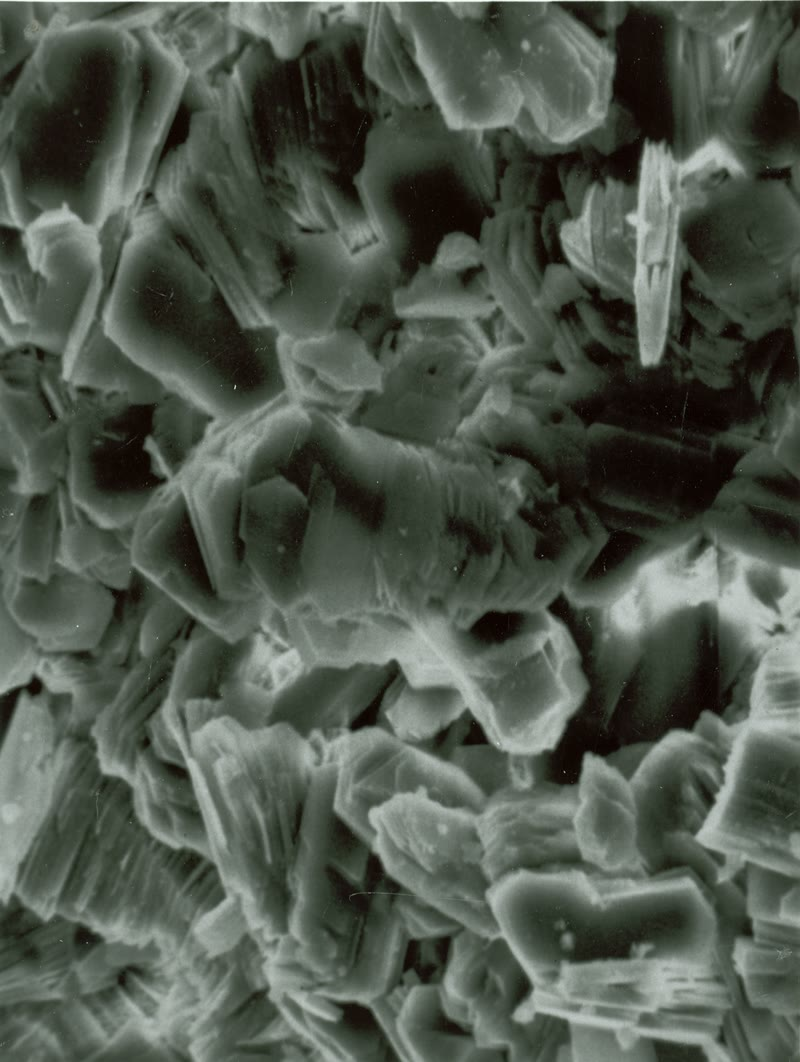
\includegraphics[width=\linewidth]{images/book3/b1-kaolinite-sem.jpg}

{\scriptsize 扫描电子显微镜下的\omterm{def:b1:weathering-clays:clay-mineral}{高岭石}：呈“书册”状的
堆叠六方片状晶体，生长于阿拉斯加北部一砂岩的孔隙中
（放大倍数约 1340 倍）。美国地质调查局，公有领域，经
维基共享资源提供。\par}
\end{minipage}
\end{omfigure}
% ledger: biscaye:1965, usgs:clay-settings, pedron:stages, commons:kaolinite-sem

\emph{\omterm{def:b1:weathering-clays:laterite}{红土}。}\omterm{def:b1:weathering-clays:hydrolysis}{水解}长期进行至最后阶段时，
剖面不断增厚，其顶部富集了一切不被带走的物质。

\begin{definition}[红土]\label{def:b1:weathering-clays:laterite}
称\emph{红土}\index{红土}为富含铁与铝的产物，
在湿热气候下强烈而持久的\omterm{def:b1:weathering-clays:hydrolysis}{水解}作用之产物：一种红色至褐色的
物质，质软或已硬化，由\omterm{def:b1:weathering-clays:clay-mineral}{高岭石}及铁的氧化物和氢氧化物构成，
达到\omterm{def:b1:weathering-clays:hydrolysis-degree}{铝铁化}阶段时还含三水铝石；其中几乎所有碱金属
和碱土金属阳离子以及大部分二氧化硅均已被移除。
\end{definition}
% ledger: formoso:laterite, buchanan:laterite

富含三水铝石或勃姆石（铝的氢氧化物）的\omterm{def:b1:weathering-clays:laterite}{红土}，即为
铝土矿，是九成以上铝的矿石：\omterm{def:b1:weathering-clays:hydrolysis-degree}{铝铁化}正是促成
矿石形成的一步。大多数铝土矿属残积型，即母岩中除氧化铝外的一切成分
都已被淋滤移走；由三水铝石构成的铝土矿多位于
热带，而且许多仍在形成之中。
% ledger: usgs:bauxite

\begin{history}[来自野外的一词]
于 1807 年，弗朗西斯·布坎南在印度南部的马拉巴尔旅行时，描述了
一种布满孔洞、富含红色与黄色铁赭石的物质，成片地
覆盖在花岗岩上，成大块分布。挖出地面时，它软到
小刀即可切开，当地人将其加工成块；在空气中，它很快
变得和砖一样硬，而且比他见过的任何砖都更耐用。当地
语言称其为“砖石”，他提议将其命名为 laterite，此名
此后地质学便用此名指热带风化形成的红色产物。
\end{history}
% ledger: buchanan:laterite

\section{硅酸盐风化与二氧化碳}\label{sec:b1:weathering-clays:co2}

\omterm{def:b1:weathering-clays:hydrolysis}{水解}产生的氢离子主要来自二氧化碳，因此将其写成碳酸，
可以看出风化对空气的作用。以硅酸钙为例，
为简便起见，记为 \ce{CaSiO3}，
\[
  \ce{CaSiO3 + 2 CO2 + H2O -> Ca^2+ + 2 HCO3- + SiO2},
\]
而在海洋中，生物用碳酸钙构筑外壳，
\[
  \ce{Ca^2+ + 2 HCO3- -> CaCO3 + CO2 + H2O}.
\]

\begin{proposition}[风化与二氧化碳]\label{prop:b1:weathering-clays:co2}
(a) 风化硅酸盐时，每释放一摩尔钙或镁，就消耗两摩尔二氧化碳，并转化为碳酸氢根；
当钙或镁以碳酸盐形式沉淀时，
其中一摩尔二氧化碳返回空气，
另一摩尔则以碳酸盐岩的形式储存。(b) 碳酸盐岩风化时，
其碳酸盐重新沉淀，则不储存任何二氧化碳。
\end{proposition}

\begin{proof}
(a) 将上面两式相加，得 \ce{CaSiO3 + CO2 -> CaCO3 + SiO2}：
每个钙对应一个 \ce{CO2} 永久离开空气；仅由第一式即可看出消耗了两个。
镁的情形相同，只需以 \ce{Mg^2+} 代替 \ce{Ca^2+}。
(b) 方解石的溶解 \ce{CaCO3 + CO2 + H2O -> Ca^2+ + 2
HCO3-} 恰是沉淀的逆过程，两者之和为零。
\end{proof}

对于\omterm{def:b1:rock-forming-minerals:groups}{长石}，碳酸代替了
\cref{prop:b1:weathering-clays:feldspars}中的氢离子：每消耗一个 \ce{H+}，就有一个 \ce{CO2}
转化为 \ce{HCO3-}。玄武岩或辉长岩中的钙\omterm{def:b1:rock-forming-minerals:groups}{长石}因此
每摩尔消耗两摩尔二氧化碳，同时转化为\omterm{def:b1:weathering-clays:clay-mineral}{高岭石}，
\[
  \ce{CaAl2Si2O8 + 2 CO2 + 3 H2O -> Al2Si2O5(OH)4 + Ca^2+ + 2 HCO3-},
\]
并长期储存其中一摩尔。钠和钾在海底不形成碳酸盐，
因此长期储存只按所释放的钙和镁计算，
不计钠和钾。

河流将碳酸氢根带入海洋，其化学成分可用来度量通量。
根据世界大河的化学成分估算，大陆硅酸盐风化消耗的二氧化碳
每年约为 \num{11.7e12} 至
\qty{13.6e12}{mol}，合 0.14 至 0.16 十亿吨碳，其中
玄武岩风化即占 30 至 \qty{35}{\percent}。这一通量与
空气、海洋和生物之间的碳交换相比很小，但它并不逆转：
在数百万年的尺度上，它是火山释放的二氧化碳
离开大气的主要途径。由于风化在更温暖、更湿润时进行得更快，
它把空气中的二氧化碳与气候联系起来，
而气候又通过温室效应依赖于二氧化碳：
这是一种负反馈，在地质时间尺度上稳定地球的温度，
将在本科二年级分册中研究。
% ledger: dessert:silicate-co2, whk:1981

\section{练习}

\begin{exercise}[$\star$]\label{exo:b1:weathering-clays:1}
已知离子半径 \ce{K+} \qty{1.38}{\angstrom}、\ce{Fe^2+} \qty{0.78}{\angstrom}，
\ce{Fe^3+} \qty{0.645}{\angstrom} 和 \ce{Ti^4+} \qty{0.605}{\angstrom}，计算每种离子的\omterm{def:b1:weathering-clays:ionic-potential}{离子势}，
并指出其所属的场。为什么排水不良的土壤会失去铁，
而排水良好的土壤则保留铁？
% ledger: shannon:radii-b19
\end{exercise}

\begin{exercise}[$\star$]\label{exo:b1:weathering-clays:2}
四种黏土组分制成定向片后进行 X 射线衍射。A：在
\SI{14}{\angstrom} 处有一峰，经乙二醇处理移至 \SI{17}{\angstrom}，并
加热至 \SI{400}{\celsius} 后移至 \SI{10}{\angstrom}。B：在
\SI{7}{\angstrom} 处有一峰，乙二醇处理后不变，加热至
\SI{550}{\celsius} 后消失。C：在 \SI{10}{\angstrom} 处有一峰，任何处理都不使其移动。D：
在 \SI{14}{\angstrom} 处有一峰，任何处理都不使其移动。判断每种\omterm{def:b1:rock-forming-minerals:mineral}{矿物}。
% ledger: usgs:clay-xrd
\end{exercise}

\begin{exercise}[$\star$]\label{exo:b1:weathering-clays:3}
借助\cref{met:b1:weathering-clays:balance}，配平正\omterm{def:b1:rock-forming-minerals:groups}{长石} \ce{KAlSi3O8} \omterm{def:b1:weathering-clays:hydrolysis}{水解}为
\omterm{def:b1:weathering-clays:clay-mineral}{高岭石}的反应。其中钾和硅各有多大比例
进入溶液？
\end{exercise}

\begin{exercise}[$\star$]\label{exo:b1:weathering-clays:4}
(a) \qty{10}{cm^3} 处于 \qty{0}{\celsius} 的水能形成多大体积的冰？
(b) 裂隙中生长的冰在哪一温度范围内使岩石破裂，
最为有效？为什么较弱或较强的霜冻效果都不及它？
(c) 边长为 \qty{1}{m} 的花岗岩立方体被霜冻分裂成边长为
\qty{1}{cm} 的立方体：其表面积增大了多少倍？
% ledger: usgs:water-density, iapws:ice-density, wh85:frost
\end{exercise}

\begin{exercise}[$\star\star$]\label{exo:b1:weathering-clays:5}
求密度为
\qty{2600}{kg.m^{-3}} 的\omterm{def:b1:rock-forming-minerals:groups}{长石}颗粒的比表面积，颗粒视为立方体，粒径分别为 \qty{1}{cm}、\qty{1}{mm}
和 \qty{1}{\micro m}。为什么颗粒粒径对\omterm{def:b1:weathering-clays:weathering}{化学风化}速率影响如此之大，
\omterm{def:b1:weathering-clays:weathering}{物理风化}为何会
加速\omterm{def:b1:weathering-clays:weathering}{化学风化}？
\end{exercise}

\begin{exercise}[$\star\star$]\label{exo:b1:weathering-clays:6}
一吨钠\omterm{def:b1:rock-forming-minerals:groups}{长石} \ce{NaAlSi3O8}（\qty{262.22}{g.mol^{-1}}）转化为
\omterm{def:b1:weathering-clays:clay-mineral}{高岭石}（\qty{258.16}{g.mol^{-1}}）。计算所生成\omterm{def:b1:weathering-clays:clay-mineral}{高岭石}的质量、
输出二氧化硅的质量（按 \ce{SiO2} 计，\qty{60.08}{g.mol^{-1}}）以及
输出钠的质量。
% ledger: webmineral:clays-b19, ciaaw:Na
\end{exercise}

\begin{exercise}[$\star\star$]\label{exo:b1:weathering-clays:7}
某花岗岩按质量计含 \qty{0.30}{\percent} \ce{TiO2}、\qty{3.5}{\percent}
\ce{Na2O}、\qty{72}{\percent} \ce{SiO2} 和 \qty{14}{\percent} \ce{Al2O3}；其
腐岩含 \qty{0.60}{\percent} \ce{TiO2}、\qty{0.35}{\percent}
\ce{Na2O}、\qty{60}{\percent} \ce{SiO2} 和 \qty{27}{\percent} \ce{Al2O3}。
假设钛不可移动，求每千克花岗岩留下的腐岩质量，
以及钠、硅和铝的损失比例。正在进行的是哪一程度的
\omterm{def:b1:weathering-clays:hydrolysis}{水解}？
\end{exercise}

\begin{exercise}[$\star\star$]\label{exo:b1:weathering-clays:8}
利用\cref{prop:b1:weathering-clays:layer-charge}，计算
叶蜡石 \ce{Al2Si4O10(OH)2}、去掉钾的白\omterm{def:b1:rock-forming-minerals:groups}{云母} \ce{KAl2(Si3Al)O10(OH)2} 的层电荷，
贝德石层 \ce{Al2(Si_{3.5}Al_{0.5})O10(OH)2} 的层电荷以及
蒙脱石层 \ce{(Al_{1.67}Mg_{0.33})Si4O10(OH)2} 的层电荷。哪些
能够膨胀？为什么？
% ledger: webmineral:clays-b19
\end{exercise}

\begin{exercise}[$\star\star$]\label{exo:b1:weathering-clays:9}
镁\omterm{def:b1:rock-forming-minerals:groups}{橄榄石} \ce{Mg2SiO4} 的风化反应为
\ce{Mg2SiO4 + 4 CO2 + 4 H2O -> 2 Mg^2+ + 4 HCO3- + H4SiO4}。(a) 检验该
方程式。(b) 对于一吨镁\omterm{def:b1:rock-forming-minerals:groups}{橄榄石}，计算所消耗的二氧化碳量，
以及依据
\cref{prop:b1:weathering-clays:co2}，计算长期封存的二氧化碳量。(c) 同样的计算
对一吨方解石将得到多少？
% ledger: ciaaw:Mg, ciaaw:Si, ciaaw:O, ciaaw:C
\end{exercise}

\begin{exercise}[$\star\star\star$]\label{exo:b1:weathering-clays:10}
(a) 电荷为 3 的离子，其半径位于何范围时为\omterm{def:b1:weathering-clays:hydrolysis}{水解}产物？(b) 硼
\ce{B^3+}，半径为 \qty{0.27}{\angstrom}：它在水中以何种形式迁移？
(c) \ce{Mn^2+} 的半径为 \qty{0.83}{\angstrom}，\ce{Mn^4+} 的
半径为 \qty{0.53}{\angstrom}。解释为何贫氧的泉水
涌入空气时会形成黑色的氧化锰结壳。(d) 为何硅既不能被完全浸出，
也不能被完全保留？
% ledger: shannon:radii-b19, nomad:goldschmidt
\end{exercise}

\begin{exercise}[$\star\star\star$]\label{exo:b1:weathering-clays:11}
大陆硅酸盐的风化每年消耗 \num{11.7e12} 至
\qty{13.6e12}{mol} 二氧化碳，其中 \qty{4.08e12}{mol} 来自
玄武岩。(a) 将该范围换算为每年的吨碳和吨二氧化碳，
(b) 玄武岩所占的份额是多少？(c) 若这些全部来自钙
和镁的硅酸盐，则每年长期封存的碳量为多少？
实际的长期量为何较小？
% ledger: dessert:silicate-co2, ciaaw:C, ciaaw:O
\end{exercise}

\begin{exercise}[$\star\star\star$]\label{exo:b1:weathering-clays:12}
三种黏土组分（已除去石英和铁氧化物）经分析（质量
百分数）：A，\ce{SiO2} \num{46.55} 和 \ce{Al2O3} \num{39.50}；B，\ce{SiO2} 60 和
\ce{Al2O3} 25；C，\ce{SiO2} 2 和 \ce{Al2O3} 63（\ce{SiO2}
\qty{60.08}{g.mol^{-1}}，\ce{Al2O3} \qty{101.96}{g.mol^{-1}}）。计算
各自的摩尔比 Si/Al，判断其所反映的\omterm{def:b1:weathering-clays:hydrolysis}{水解}程度，并
将三种土壤按浸出强度从弱到强排列。
% ledger: webmineral:clays-b19, pedron:stages, formoso:laterite
\end{exercise}

\section{问题：从花岗岩到黏土}

\begin{problem}[{周末问题——花岗岩与辉长岩中的长石，从
配平的反应到河流带走的二氧化碳}]
\label{pb:b1:weathering-clays:1}
% values: calc/ch19.py; the river is invented (its numbers are of a realistic order)
\omterm{def:b1:rock-forming-minerals:groups}{长石}包括钠\omterm{def:b1:rock-forming-minerals:groups}{长石} \ce{NaAlSi3O8}（\qty{262.22}{g.mol^{-1}}，密度
\qty{2.62}{g.cm^{-3}}）和钙\omterm{def:b1:rock-forming-minerals:groups}{长石} \ce{CaAl2Si2O8}
（\qty{278.20}{g.mol^{-1}}，密度 \qty{2.75}{g.cm^{-3}}）。\omterm{def:b1:weathering-clays:clay-mineral}{高岭石}
\ce{Al2Si2O5(OH)4} 的摩尔质量为 \qty{258.16}{g.mol^{-1}}，密度
为 \qty{2.6}{g.cm^{-3}}；三水铝石 \ce{Al(OH)3}，\qty{78.00}{g.mol^{-1}}。取
\ce{SiO2} \qty{60.08}{g.mol^{-1}}，\ce{CO2} \qty{44.01}{g.mol^{-1}}，\ce{HCO3-}
\qty{61.02}{g.mol^{-1}}，Na \num{22.99} 和 Ca \qty{40.08}{g.mol^{-1}}。
% ledger: hom:albite, hom:anorthite, webmineral:clays-b19, ciaaw:Na, ciaaw:Ca, ciaaw:C, ciaaw:O, ciaaw:H

\medskip
\noindent\textbf{第一部分——反应式。}
\begin{enumerate}
  \item 配平钠\omterm{def:b1:rock-forming-minerals:groups}{长石}\omterm{def:b1:weathering-clays:hydrolysis}{水解}生成\omterm{def:b1:weathering-clays:clay-mineral}{高岭石}的反应。
  \item 配平钙\omterm{def:b1:rock-forming-minerals:groups}{长石}\omterm{def:b1:weathering-clays:hydrolysis}{水解}生成\omterm{def:b1:weathering-clays:clay-mineral}{高岭石}的反应。该反应有何
        特殊之处？
  \item 配平钙\omterm{def:b1:rock-forming-minerals:groups}{长石}\omterm{def:b1:weathering-clays:hydrolysis}{水解}生成三水铝石的反应。
  \item 配平钠\omterm{def:b1:rock-forming-minerals:groups}{长石}\omterm{def:b1:weathering-clays:hydrolysis}{水解}生成贝德石
        \ce{Na_{0.5}Al2(Si_{3.5}Al_{0.5})O10(OH)2} 的反应，并核对氢的平衡。
  \item 以碳酸作为氢离子的来源，改写前两个反应，
        其中氢离子由 \ce{CO2 + H2O -> H+ + HCO3-} 提供。
  \item 其中哪些反应属于\omterm{def:b1:weathering-clays:hydrolysis-degree}{双硅铝化}、\omterm{def:b1:weathering-clays:hydrolysis-degree}{单硅铝化}和
        \omterm{def:b1:weathering-clays:hydrolysis-degree}{铝铁化}？
\end{enumerate}

\medskip
\noindent\textbf{第二部分——留存与流失。}
\begin{enumerate}[resume]
  \item 一吨钠\omterm{def:b1:rock-forming-minerals:groups}{长石}和一吨
        钙\omterm{def:b1:rock-forming-minerals:groups}{长石}各含多少摩尔？
  \item 计算由每吨\omterm{def:b1:rock-forming-minerals:groups}{长石}所生成的\omterm{def:b1:weathering-clays:clay-mineral}{高岭石}质量。
  \item 计算以溶液形式输出的二氧化硅（以 \ce{SiO2} 计）、钠和钙
        的质量。
  \item 计算每吨各\omterm{def:b1:rock-forming-minerals:groups}{长石}及其所生成的\omterm{def:b1:weathering-clays:clay-mineral}{高岭石}体积。
        固体体积缩小的比例是多少？
  \item 腐岩保持所替代岩石的形状。在富含钠\omterm{def:b1:rock-forming-minerals:groups}{长石}的风化花岗岩中，
        留下的空间由什么填充？为什么富含钙\omterm{def:b1:rock-forming-minerals:groups}{长石}的风化辉长岩
        仍然更致密？
  \item 利用\omterm{def:b1:weathering-clays:ionic-potential}{离子势}图，解释两种\omterm{def:b1:rock-forming-minerals:groups}{长石}中的哪些元素
        会流失、哪些保留。
\end{enumerate}

\medskip
\noindent\textbf{第三部分——二氧化碳。}
\begin{enumerate}[resume]
  \item 一吨钠\omterm{def:b1:rock-forming-minerals:groups}{长石}转变为\omterm{def:b1:weathering-clays:clay-mineral}{高岭石}时，消耗的二氧化碳
        为多少摩尔、多少千克？
  \item 对一吨钙\omterm{def:b1:rock-forming-minerals:groups}{长石}提出同样的问题。
  \item 钙\omterm{def:b1:rock-forming-minerals:groups}{长石}输出的碳酸氢盐质量为多少？
  \item 这些碳酸氢盐在海洋中发生什么变化？有多少
        所消耗的二氧化碳重新回到大气中？
  \item 为什么不计算钠\omterm{def:b1:rock-forming-minerals:groups}{长石}中钠的长期封存量？
  \item 将其与一吨方解石的溶解及随后的
        沉淀过程进行比较。
\end{enumerate}

\medskip
\noindent\textbf{第四部分——一条河流。}
\begin{enumerate}[resume]
  \item 一条河流的流域面积为 \qty{50000}{km^2}，覆盖花岗岩和片麻岩，
        平均流量为 \qty{200}{m^3.s^{-1}}，河水所携带的
        由硅酸盐风化产生的碳酸氢盐浓度为 \qty{0.3}{mmol.L^{-1}}。计算该碳酸氢盐的年通量，
        以摩尔计，并以每平方千米为单位。
  \item 将其表示为钙\omterm{def:b1:rock-forming-minerals:groups}{长石}的摩尔数，即风化为
        \omterm{def:b1:weathering-clays:clay-mineral}{高岭石}时可提供该量的钙\omterm{def:b1:rock-forming-minerals:groups}{长石}；再以每年的吨数表示，
        并以每平方千米计。
  \item 若岩石中相当于含 \qty{20}{\percent} 的钙\omterm{def:b1:rock-forming-minerals:groups}{长石}，
        且密度为 \qty{2700}{kg.m^{-3}}，则新鲜岩石被消耗的速率为
        每百万年多少米？
  \item 这条河流每年从大气中永久移除多少
        二氧化碳？
  \item 为何第 21 题的速率是地表降低的
        下限？
  \item 以千克为单位，取三位有效数字，计算
        一吨钙\omterm{def:b1:rock-forming-minerals:groups}{长石}风化所永久汲取的二氧化碳量是多少？
\end{enumerate}
\end{problem}
